\documentclass[10pt]{article}

\usepackage{wrcecapstone}
\hypersetup{
  pdfauthor={Chris Ashley, Graham Brothers, and Cameron Douglas},
  pdftitle={TurtleBot},
  pdfsubject={weapons, robotics, and control engineering},
  pdfkeywords={biomechanics, sea turtle, amphibious, flapping foil}
}
\coursenumber{EW401}
\student{MIDN 1/C G.~AShley, MIDN 1/C G.~Brothers, and MIDN 1/C C.~Douglas}
\advisor{Assistant Professor D. Evangelista}


\title{TurtleBot}
\author{MIDN 1/C G Ashley, G Brothers, and C Douglas}
\date{\printdate{12/3/2020}}

\begin{document}
\maketitlepage
\cleardoublepage
\tableofcontents
%\listoffigures
%\listoftables

%first page
\clearpage
\maketitle
\begin{abstract}
Your abstract should summarize the objective of your capstone project, briefly explain its importance in context of the broader engineering landscape, summarize the final design and highlight significant results or performance measures.
\end{abstract}

\section{1. Introduction}
\subsection{1.1. Customer Interview}
Our customer is Dr. William Sandberg, who is currently a professor at George Mason University and a maritime research specialist. He works with RDSA and has experience in foils and fins as they relate to our project. Depending on the success of our project, one of his potential plans for our product is to forward the design to government contractors for further development or research purposes. He will also potentially use this in his own research or instruction. The highlights from our interview include the matriculation and application our project will have, the difficulty of waterproofing, the material of the fins and outer body, an advised timeline, and greater insight on the movement of the fins. We found that these types of projects are the foundation of work much later that sees real application and use. Waterproofing came up as a serious risk in terms of the design feasibility of our project, we came to the conclusion modularity needs to take priority in our design to combat the difficulty of waterproofing. We found that through our consultation the opportunities for design are not limited due to the resources at our disposal to create inexperienced materials/ components for our project. We came to the conclusion that in order to effectively design our bot we need to structure the design process to effectively incorporate modularity and a process of feedback. Finally we were advised on various prevalent research that will be useful in our design of our finned bot. Our point of view statement is: A mission platform conducting surface or undersea operations needs to be able to maneuver a deployed UAV accurately at low speeds in order to recover them in a way that is much safer and cost-effective than the current means. 

\subsection{1.2. Additional Background Research}
Historically autonomous underwater vehicles have followed commonly accepted forms of propulsion, to include conventional propeller controlled UUVs. These systems have limitations in their mission scope due to capabilities they possess to include lack of low speed maneuverability and inherent limitation of these vehicles to transition from the aquatic environment to that of the terrestrial. These lack of features in conventional robotic systems present a need for significant advancement of technology and design of UUVs. Researchers can turn towards living organisms for inspiration to design energy efficient propulsion systems with high maneuverability and amphibious capabilities, 550 million years of evolution has given us numerous sources to draw ideas from. As Dr. Stephen Carl Licht a researcher at MIT put it “To push the operating range of underwater vehicles, particularly small autonomous robots, into these chaotic margins we must close the performance gap between nature and machine” Many organisms to include; sea turtles, seals and penguins for example all have amphibious capabilities and low speed maneuverability each however has achieved this capability with its own unique design. Our research presents three projects which will explore the idea of drawing on nature as a resource in the design and advancement of technology of UUVs. 

The first project explored biomimetic oscillating foil propulsion to enhance underwater vehicle agility and maneuverability. The Licht Turtlebot, designed by MIT researcher Dr. Stephen Carl Licht and his team designed an autonomous underwater vehicle (AUV) inspired by the swimming abilities of sea turtles powered by four fins. Through the use of biometric actuation this project has improved the maneuverability of AUVs, particularly in its ability to both maneuver at cruising speeds and remain agile at lower speeds. The 2nd project explored system integration and fin trajectory design for a robotic sea-turtle. The Naro-Tartaruga bot team designed a robotic platform which utilizes fin propulsion actuators that imitate a sea-turtle while implementing basic concepts of control for fin locomotion. As described by the Naro-Tartaruga bot team this project's motivation was “the fluent and aesthetic locomotion of marine animals... Flexibility, agility, efficiency, high speeds, and endurance are some of the main attributes that can be used to describe fin-locomotion concepts.” The 3rd project explored flipper-driven terrestrial locomotion of a sea turtle-inspired robot. The Flipper Bot team through the study of hatchling sea turtles design a robotic platform to mimic the territorial based locomotion of hatchling sea turtles.  As described by the FlipperBot team this project's motivation was “To discover principles of flipper-based terrestrial locomotion we study the mechanics of a hatchling sea turtle-inspired robot [1]” The purpose of each of these projects was to further the technology and design of amphibious vehicles through the study of nature.

\section{2. Problem Statement}
\subsection{2.1. Problem Statement}
To develop and design an amphibious vehicle that is able to accurately maneuver at low speeds in still water, crawl in a variety of water depths, and transition  from the locomotion of swimming to crawling seamlessly utilizing locomotion of sea turtles as inspiration.
\subsection{2.2. Functions}
Our functionality requirements, in hierarchical order, are as follows: must be able to move forward in the water, must be able to turn left and right in the water, must be able to move forward on land, must be able to turn left and right on land, and must be able to crab left and right in the water.
\subsection{2.3. Constraints}
Our robot needs to operate under a certain power threshold – the quantity is yet to be determined. Our robot also must withstand up to 15 feet of water pressure. Our robot needs to fit within certain dimensions to help the design process and functionality. Additionally, our robot needs to operate regularly with zero mechanical failures. 
\subsection{2.4. Objectives, Pairwise Comparison Chart, and Weightings}

\begin{figure}
\caption{Objectives, PCC and weightings}
\label{fig:obj}
\end{figure}
%Must be able to move forward on land
%Must be able to move forward in the water
%Must be able to turn left and right in the water
%Must be able to turn left and right on land 
%Must be able to crab left and right in the water
%Score
%Decision matrix weights
%Must be able to move forward on land
%**
%0
%0
%1
%1
%2
%3
%Must be able to move forward in the water
%1
%**
%1
%1
%1
%4
%5
%Must be able to turn left and right in the water
%0
%0
%**
%1
%1
%2
%3
%Must be able to turn left and right on land 
%0
%0
%0
%**
%1
%1
%2
%Must be able to crab left and right in the water
%0
%0
%0
%0
%**
%0
%1
%
%
%
%Accurately maneuvers
%Transitions seamlessly
%
%Inexpensive
%
%Controllable
%
%Maintainable /Reliable
%
%Score
%Decision matrix weights
%Accurately maneuvers
%**
%1
%1
%0
%1
%3
%4
%Transitions seamlessly
%0
%**
%1
%0
%1
%2
%3
%Inexpensive
%0
%0
%**
%0
%1
%1
%2
%Controllable
%1
%1
%1
%**
%1
%4
%5
%Modularity
%0
%0
%0
%0
%**
%0
%1
%

\subsection{2.5. Metrics}
\begin{figure}
\caption{Metrics}
\label{fig:metrics}
\end{figure}
%Mobility in water
%Score
%Metric
%4
%Swim at speeds of 1 body length of the robot per second
%3
%Swim at speeds of 3/4 body length of the robot per second
%2
%Swim at speeds of 1/2 body length of the robot per second
%1
%Swim at speeds of 1/4 body length of the robot per second
%0
%Is not able to swim 
%
%
%Mobility on land
%Score
%Metric
%4
%Crawl at speed of 1/3 body length of the robot per second
%3
%Crawl at speed of 1/4 body length of the robot per second
%2
%Crawl at speed of 1/6 body length of the robot per second
%1
%Crawl at speed of 1/10 body length of the robot per second
%0
%Is not able to crawl
%
%
%
%
%
%
%
%
%
%
%
%Amphibious Capability
%Score
%Metric
%4
%Operate in shallow water level 10% of height of the robot, transition from water to land seamlessly 
%3
%Operate in shallow water level 7% of height of the robot, transition from water to land is labored
%2
%Operate in shallow water level 5% of height of the robot, regularly able to transition water to land
%1
%Irregularly able to transition from water to land 
%0
%Cannot operate in any amphibious fashion and unable to transition from water to land 
%
%
%Simplicity 
%Score
%Metric
%4
%Uses less than 8 of same motors , the fins all the same, and the shoulder/leg mechanisms are the same 
%3
%Uses less than 8 motors with multiple types of motors, the fins are the same, and the  shoulder leg/mechanism are the same 
%2
%Uses less than 8 motors with multiple types of motors, the fins are the different, and the shoulder leg/mechanism are the same 
%1
%Uses less than 10 motors with multiple types of motors, the fins are the different, and the shoulder leg/mechanism are the same 
%0
%Uses less than 10 motors with multiple types of motors, the fins are the different, and the shoulder leg/mechanism are different 

\section{3. Related Work}
The Licht Turtlebot \cite{licht2008biomimetic}, designed by MIT researcher Dr. Stephen Carl Licht, features biometric oscillating foil propulsion to enhance underwater vehicle agility and maneuverability. The robot has numerous features we hope to emulate, as well as shortcomings to improve upon. Its strengths include: Highly agile at low speeds, highly maneuverable at cruising speeds, and it is built for swimming and very high performing in that category. Its weaknesses are: The actuators do not allow for travel on land, it does not have enough degrees of freedom for our movement, and its large scale requires more power and manpower to operate. 

The Naro Tartaruga Bot \cite{siegenthaler2013system} is another related project. This turtlebot consists of four flapping foils, two pectoral fins and two rear fins, and eight sensors, to include a pressure sensor, temperature sensor, GPS, gyro, compass, encoders, and water leakage/flow sensors. The fins have three degrees of freedom, allowing for greater mobility and maneuverability. Its strengths include that it will very closely resemble the locomotion of a Sea Turtle, which is our end goal. It will also provide unique means of maneuvering that may prove much more agile, efficient, and smooth. Its main weakness is having different size fins with irregular shapes may pose a problem with creating the optimal speed and sweeping angles to achieve the proper movement patterns.

The Flipperbot \cite{mazouchova2013flipper} is a two-limbed robot operated by dual servo motors connected to a hull-mounted bending shoulder mechanism. It was designed to test flipper-based terrestrial locomotion. Its strengths include a simple mechanical design and its proven example for sustained travel on land. However, it is unable to efficiently travel in water like other models. 

The purpose of each of these projects was to further the technology and design of amphibious vehicles through the study of nature. Our robot design needs swimming capabilities, terrestrial locomotion with flippers, and proper system integration and fin trajectory. Collectively, these projects provide examples of all our necessary features. 

\section{4. Conceptual Designs}
\subsection{4.1. Design Concept 1:} 
Inner mechanics - There will be only a microprocessor and sensors to include an IMU.  As communications and power will be achieved through the use of tethering. 

Fins - Will be unique in form in comparison per set of pectoral and lower fins, they will be constructed of a semi-stiff composite plastic. They will be larger in comparison to the scale depicted in the drawing to the left. 

Outer body - Will be constructed of stiff composite plastic that will add buoyancy if needed, another layer of waterporectection, and make the turtlebot have less hydrodynamic drag. 

Shoulder mechanism - Composed of two servo motors connected to a dc motor contained in a stationary. This will allow the front flippers to both be able to properly replicate the locomotive  gait of the pectoral fins of sea turtle swimming while also enabling the flippers to aid in crawling .

Leg mechanism - Composed of three servo motors connected in conjunction to the body of turtle bot. The three servos will allow these flippers to aid in providing thrust for swimming and enable the locomotive terrestrial gait of sea turtles.   

Means 1
Means 2
Means 3
Locomotion in water 
Combination of servo and DC motors in shoulder and leg mechanisms 
DC motors in shoulder and leg mechanisms
Servo motors in shoulder and leg mechanisms
Locomotion on land 

Two servos motors in shoulder mechanism connected in linkage 
Three servos motors in shoulder mechanism connected in linkage 
Two servos and DC motor shoulder mechanism connected in linkage 
Power supply 
Powered completely within bot ( Lithium Ion batteries )
Power tethered to the bot 
**
Outer body 
Rigid Composite plastic 
Soft composite plastic
**
Communication
 And Control
Microcontroller contained with bot/ communications tethered to bot
Everything contained within bot 
**
Fins 
Rigid Composite plastic
Passively deformable material (leading edge stiffer than trailing) 
Fin system that allows the fin to be flexible or rigid upon command 

\subsection{4.2. Design Concept 2:}

Inner mechanics - There will need to be many mechanics contained within a watertight seal in the turtlebot to include microprocessor, battery, wireless connector, circuit board, and relevant sensors to include an IMU.

Leg and shoulder mechanism - Composed of two servo motors connected in conjunction to the body of turtle bot. The two servos will allow these flippers to aid in providing thrust for swimming and enable the locomotive terrestrial gait of sea turtles.  

Fins - All four fins will be the same dimensions and they will be constructed of a semi flexible plastic that allows the fin to be flexible or rigid when needed . They will be larger in comparison to the scale depicted in the drawing to the left. 


Means 1
Means 2
Means 3
Locomotion in water 
Combination of servo and DC motors in shoulder and leg mechanisms 
DC motors in shoulder and leg mechanisms
Servo motors in shoulder and leg mechanisms
Locomotion on land 

Two servos motors in shoulder mechanism connected in linkage 
Three servos motors in shoulder mechanism connected in linkage 
Two servos and DC motor shoulder mechanism connected in linkage 
Power supply 
Powered completely within bot ( Lithium Ion batteries )
Power tethered to the bot 
**
Outer body 
Rigid Composite plastic 
Soft composite plastic
**
Communication
 And Control
Microcontroller contained with bot/ communications tethered to bot
Everything contained within bot 
**
Fins 
Rigid Composite plastic
Passively deformable material (leading edge stiffer than trailing) 
Fin system that allows the fin to be flexible or rigid upon command 

\subsection{4.3. Design Concept 3:}
Inner mechanics - There will need to be many mechanics contained within a watertight seal in the turtlebot to include microprocessor, battery, wireless connector, circuit board, and relevant sensors to include an IMU.
Outer body - Will be constructed of soft composite plastic that will add buoyancy if needed, another layer of water protection, and make turtlebot have less hydrodynamic drag. 
Leg and shoulder mechanism - Composed of three servo motors connected in conjunction to the body of turtle bot. The three servos will allow these flippers to aid in providing thrust for swimming and enable the locomotive terrestrial gait of sea turtles.

Means 1
Means 2
Means 3
Locomotion in water 
Combination of servo and DC motors in shoulder and leg mechanisms 
DC motors in shoulder and leg mechanisms
Servo motors in shoulder and leg mechanisms
Locomotion on land 

Two servos motors in shoulder mechanism connected in linkage 
Three servos motors in shoulder mechanism connected in linkage 
Two servos and DC motor shoulder mechanism connected in linkage 
Power supply 
Powered completely within bot ( Lithium Ion batteries )
Power tethered to the bot 
**
Outer body 
Rigid Composite plastic 
Soft composite plastic
**
Communication
 And Control
Microcontroller contained with bot/ communications tethered to bot
Everything contained within bot 
**
Fins 
Rigid Composite plastic
Passively deformable material (leading edge stiffer than trailing) 
Fin system that allows the fin to be flexible or rigid upon command 

\subsection{4.4. Decision Matrix}
%Decision Matrix :Design Constraints (C)
% &
%Objectives (O)
%Weight
%Design Concept 
%one 
%Design Concept 
%two
%Design Concept Three
%Low power (C)
%**
%Yes
%Yes
%Yes
%Waterproof(C)
%**
%Yes
%Yes
%Yes
%Small Size (C)
%**
%Yes
%Yes
%Yes
%Durable(C)
%**
%Yes
%Yes
%Yes
%Controllable(O)
%5
%15/20 -75
%11/20 - 55
%8/20-40
%Maneuverable(O)
%4
%12/16 - 48
%7/16- 28
%12/16-48
%Beach Transition(O)
%3
%9/12 - 27
%4/12 -12
%11/12- 33
%Modularity(O)
%1
%8/12 - 8
%7/12- 7
%5/12-5
%Inexpensive(O)
%2
%1/8 - 2
%5/8- 10
%2/8- 4
%Total
%**
%160
%112
%130
%
Our winning design is Design Concept One. It was ranked highest overall based on our objectives of controllability, maneuverability, beach transition, modularity, and cost. 

\section{5. Ethical Considerations}
Briefly discuss ethical issues that impacted your design approach.  Incorporate the \emph{IEEE Code of Ethics}\footnote{IEEE Code of Ethics is available online at \url{https://www.ieee.org/about/corporate/governance/p7-8.html}} or the \emph{Professional Engineer’s Code}\footnote{The NSPE Code of Ethics is availble online at \url{https://www.nspe.org/resources/ethics/code-ethics}} into your discussion when possible.

\section{6. Engineering Standards and Specifications}
Discuss an engineering standard or specification that is applicable to at least one component of your design.

\section{7. Preliminary Detailed Design}
\subsection{7.1. Component Selection}
For any components not discussed in the previous section, explain how you selected all parts such as actuators, power supplies, computing resources, and sensors include a morph chart.  Provide engineering justifications for your choices.
 
\subsection{7.2. Parts List and Budget}

\subsection{7.3. Mechanical Drawings}
Include dimensioned drawings of parts you plan on building or having the shop fabricate.   Neat hand drawings are acceptable. 
\begin{figure}
\caption{This is an example of a dimensioned mechanical drawing (left) and an annotated photo (right).  This caption was created using the \lstinline{\\caption} command. Fuck MS Word.}
\label{fig:1}
\end{figure}

\subsection{7.4. Circuit Diagrams}
Provide circuit diagrams of any electronics subsystems you will build.
\begin{figure}
\caption{Circuit diagram}
\label{fig:2}
\end{figure}

\subsection{7.5. Prototypes}
Show pictures of any prototypes or scale models you made.

\subsection{7.6. Software Structure}
Your algorithm or controller design should be in the format of pseudo-code (see Figure 3). It is not necessary to include computer programs in their entirety, though interesting excerpts may be included in the text. Appropriately comment any included code. The documentation needs to clearly indicate what code was written by the group members versus code provided by another source (e.g. faculty, TSD, commercial or open-source software, etc.).  For larger, hierarchical programs, represent the functional organization with a flow chart or a block diagram.  For programs utilizing GUIs, screen captures of the user interface are useful.   
\begin{figure}
\caption{Pseudo-code is one of the most compact ways to present computer programs. Code is included using the \texttt{listings} package.}
\label{fig:3}
\end{figure} 

\subsection{7.7. Simulations}
This section could include the development of a mathematical model and/or the use of a model to predict behavior and system performance.  If you used simulation or other computer-aided design tools discuss them here. 
\begin{figure}
\caption{This is the response of the feedback control law.   Note that it is scaled appropriately to see the interesting features, and annotated.   When importaing Matlab figures, you may need to increase the font size and line width using Matlab to improve legibility.}
\label{fig:5} %???
\end{figure}

\section{8. Proposed Work}
\subsection{8.1. Work Breakdown Structure}
\subsection{8.2. Timeline}
\subsection{8.3. Risk management}
When working with various power systems and equipment with high amounts of current, we will need to handle with care. This is especially true when we are working with electronics in the water. Additionally, while constructing our robot, we will need to use safety gear and handle with extreme care. Safety glasses and gloves will be worn at all times when machinery is being operated. 

\subsection{8.4. Demonstration and Testing Plan}
Discuss your approach to testing your project, broken down by sub-system.
Explain in detail how the metrics will be evaluated. 

\section{9. Benchtop Demonstration}
Our Bench Demonstration will consist of a working tetrix and 3D printed TurtleBot capable of crawling. The robot will be composed of: 6 Hobby Servos, an Mbed Microcontroller, a 6V power source, a breadboard, 4 3D printed clamp linkages, and 3D printed fins. 

\subsection{9.1. Activities}
Describe the activities you engaged in during the final weeks of the semester.

\subsection{9.2. Results}
Present the results of your benchtop testing. 

%References
%Instructions on how to insert references in MS Word appear in the Appendix.  The following examples show how most common materials should be referenced using the IEEE standard. Note: parenthetical descriptions should not be included in your reference entries.
%[1] 	N. Mazouchova, P. B. Umbanhowar, and D. I. Goldman, “Flipper-driven terrestrial locomotion of a sea turtle-inspired robot,” Bioinspiration & Biomimetics, vol. 8, no. 2, p. 026007, 2013. 
%[2]	S. C. Licht, “Biomimetic oscillating foil propulsion to enhance underwater vehicle agility and maneuverability,” 2008. 
%[3]	 C. Siegenthaler, C. Pradalier, F. Gunther, G. Hitz, and R. Siegwart, “System integration and fin trajectory Design for a robotic sea-turtle,” 2013 IEEE/RSJ International Conference on Intelligent Robots and Systems, 2013. 
%\nocite{*}
\bibliographystyle{IEEEtran}
\bibliography{IEEEabrv,turtlebot.bib}


\clearpage
\appendix
\section{Formatting and Style Guidelines}\label{app-style}
Appendices are optional and should appear at the end. You may have several appendices if necessary, to include computer programs, large data sets, or detailed drawings. Be sure to note the existence of any appendices or enclosures within the relevant portion of the report text.  

This appendix provides stylistic guidelines and \LaTeX\ tips on creating linked and cross referenced documents.  

\subsection{Abbreviations and Acronyms}
Define abbreviations and acronyms the first time they are used in the text, even after they have been defined in the abstract. Abbreviations such as IEEE, SI, MKS, CGS, ac, dc, and rms do not have to be defined. Do not use abbreviations in the title or heads unless they are unavoidable.

\subsection{Units}
The use of SI units is encouraged. English units may be used as secondary units (in parentheses). An exception would be the use of English units as identifiers in trade, such as ``3.5-inch disk drive''. Use a zero before decimal points: ``0.25'', not ``.25''. Use ``\si{\centi\meter\cubed}'', not ``cc''. In \LaTeX, you can use the \lstinline{siunitx} package to ensure units are done correctly. 

\subsection{Equations}
\LaTeX will automatically number equations consecutively. Equation numbers, within parentheses, are to position flush right, as in (\ref{eq2}). Punctuate equations with commas or periods when they are part of a sentence, as in
\begin{equation}
\alpha + \beta = \chi.
\label{eq2}
\end{equation}
Note that the equation is centered. Be sure that the symbols in your equation have been defined before or immediately following the equation. For IEEE format, use ``(\ref{eq2})'', not ``Eq. (\ref{eq2})'' or ``equation (\ref{eq2})'', except at the beginning of a sentence: ``Equation (\ref{eq2}) is ...''For non-IEEE formats, equation~\ref{eq2} is sufficient. 

\subsection{Figures and Tables}
Place figures and tables at the top and bottom of pages. Avoid placing them in the middle of pages. Figure captions should be below the figures as shown in Figure~\ref{f6}; table captions should appear above the tables as shown Table~\ref{t1}. In \LaTeX, the environments to include figures and tables are \lstinline{figure} and \lstinline{table}, respectively (together they are sometimes called ``floats''). 

To insert captions, use the \lstinline{caption} command within the body of your figure or table.  After the caption, provide a \lstinline|\label{labelname}| that you will use to refer to the figure.  Reference the figure in the text by using the text \lstinline|\ref{labellname}|.  This also works for referring to other sections of the text, etc. 

\begin{table}[hpt]
\caption{Captioned Table}
\label{t1}
\begin{center}
\begin{tabular}{lcc}
\toprule
 & col1 & col2 \\
\midrule
row1 & 1 & 2 \\
row2 & 3 & 4 \\
\bottomrule
\end{tabular}
\end{center}
\end{table}

\begin{figure}[hpb]
\begin{center}
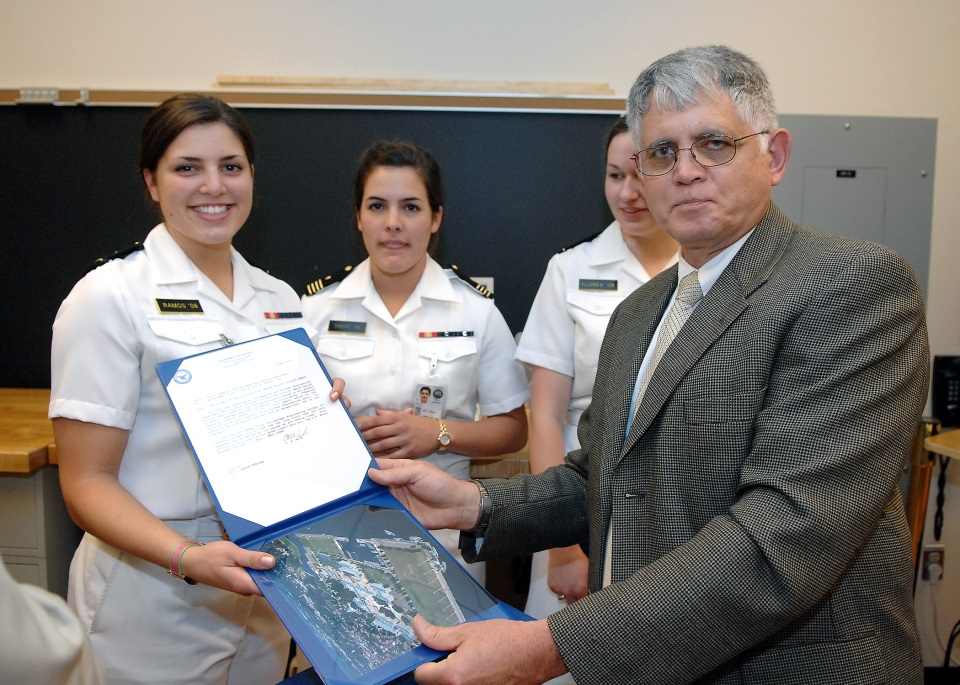
\includegraphics{figures/f6.png}
\end{center}
\caption{Presentation of the 2007 Marsh Award, which is given each year to the best 1/C Systems Engineering project in memory of ENS David R.  Marsh, USNA Class of 1987, in honor of his enthusiasm for his 1/C project, a voice activated robot.}
\label{f6}
\end{figure}

When composing your figures in Inkscape or Adobe Illustrator, use 8 point Arial or Times New Roman for axis label or titles. Use words rather than symbols or abbreviations to avoid confusing the reader. As an example, write the quantity ``Magnetization'', or ``Magnetization, $M$'', not just ``$M$''. If including units in the label, present them within parentheses. Do not label axes only with units. In the example, write ``Magnetization (\si{\ampere\per\meter})'' not just ``\si{\ampere\per\meter}''. Scale the figure appropriately for one or two columns so that they are readable, with thick enough lines and markers, etc. 

With \lstinline{.svg} files, it is possible to include \LaTeX\ and to have it automatically match the font and size with the body of the text when using \lstinline{includesvg}. 

\subsection{References}
Use \lstinline{bibtex}, it's much easier than using the thing built into Word. If you enter things correctly, it will handle the formatting for you. It will also automatically and correctly number the citations. The file \lstinline{example.bib} gives examples of how to code the bibliographic entries. 

To cite them, within the body of your text use the \lstinline|\cite{refname}| command. \LaTeX\ will automatically sort, number, etc. IEEE formats use a reference number within brackets, e.g. \cite{young1964synthetic}. The format of bibliography references can be changed using the \lstinline|\bibliographystyle| command. You may wish to do so if biology-style (Author, 2018) parenthetical references are more appropriate for your subject, for example. 

\end{document}

